%!TEX encoding = UTF-8 Unicode
%!TEX root = ../doc-plm.tex





\chapter{Routines}

PLM définit plusieurs natures de routines~:
\begin{itemize}
  \item les \emph{procédures}, dont l'appel est une instruction (\refSubsectionPage{declarationProcedure})~;
  \item les \emph{fonctions}, dont l'appel est une instruction ou apparaît dans une expression (\refSectionPage{defFonction})~;
  \item les \emph{boot routines}, exécutées une fois avant l'initialisation des variables globales (\refSectionPage{bootRoutine})~;
  \item les \emph{init routines}, exécutées une fois après l'initialisation des variables globales (\refSectionPage{initRoutine})~;
  \item les \emph{routines de panique}, exécutées lors d'une panique (\refSectionPage{routinePanique})~;
  \item les routines \emph{système}, qui sont les points d'entrée des routines privilégiées à partir des routines utilisateur (\refSectionPage{declarationSystem})~;
  \item les \emph{routines d'interruption}, qui sont des primitives de l'exécutif (\refSectionPage{declarationRoutineInterruption}).
\end{itemize}


\section{Modes logiques}

À chaque routine est attaché statiquement un mode d'exécution.

La plupart des processeurs définit plusieurs modes d'exécution, typiquement un mode \emph{système} ou \emph{privilégié} (où toutes les ressources sont accessibles), et un mode \emph{utilisateur}, où certaines instructions, espace mémoire, registres de contrôles sont inaccessibles.

Cependant, un mode \emph{système} unique est trop sommaire pour reflèter toutes les natures de routines. C'est pourquoi PLM définit neuf modes de fonctionnement, \plm=user=, \plm=primitive=, \plm=service=, \plm=section=, \plm=safe=, \plm=guard=, \plm=panic=, \plm=boot= et \plm=init=, qui sont décrits ci-après.

\subsection{Définition des modes}

\plm=user=. Ce mode est le mode d'exécution des tâches. C'est le seul mode qui correspond au mode \emph{user} du processeur. Seuls les registres de contrôle déclarés avec l'attribut \plm=@user= sont accessibles. Les instructions qui peuvent engendrer une panique sont autorisées.

\plm=primitive=. Dans ce mode, les opérations de l'exécutif qui peuvent bloquer ou rendre prête une tâche sont appelables. Tous les registres de contrôle sont accessibles, et les instructions qui peuvent engendrer une panique sont autorisées. 

\plm=service=. Seule différence avec le mode précédent, les opérations de l'exécutif qui peuvent bloquer une tâche ne sont pas appelables, uniquement celles qui peuvent rendre prête une tâche le sont.

\plm=section=. Dans ce mode, on ne peut ni bloquer ni rendre prête une tâche. Ce mode permet d'exécuter des opérations de manière indivisible. Les instructions qui peuvent engendrer une panique sont autorisées.

\plm=safe=. Par rapport au mode précédent, les instructions qui peuvent engendrer une panique ne sont pas autorisées.

\plm=guard=. C'est le mode d'évaluation des commandes gardées. Les seules opérations de l'exécutif autorisées sont celles relatives aux gardes. Les instructions qui peuvent engendrer une panique sont autorisées.

\plm=panic=. Lorsqu'une instruction engendre une panique, l'exécution est déroutée vers les routines dédiées qui s'exécutent dans ce mode.  Les instructions qui peuvent engendrer une panique n'y sont pas autorisées.

\plm=boot=. C'est le mode après le démarrage du micro-contrôleur, pour le configurer. L'accès aux variables globales est interdit (elles ne sont pas encore initialisées), seul l'accès aux registres de contrôle est autorisé. Les instructions qui peuvent engendrer une panique n'y sont pas autorisées.


\plm=init=. C'est le mode d'initialisation. L'initialisation est exécutée après le \plm=boot=, l'accès aux variables globales est autorisé, ainsi que l'accès aux registres de contrôle. Les instructions qui peuvent engendrer une panique n'y sont pas autorisées.














\subsection{Changement de mode}

\begin{figure}[t]
  \centering
  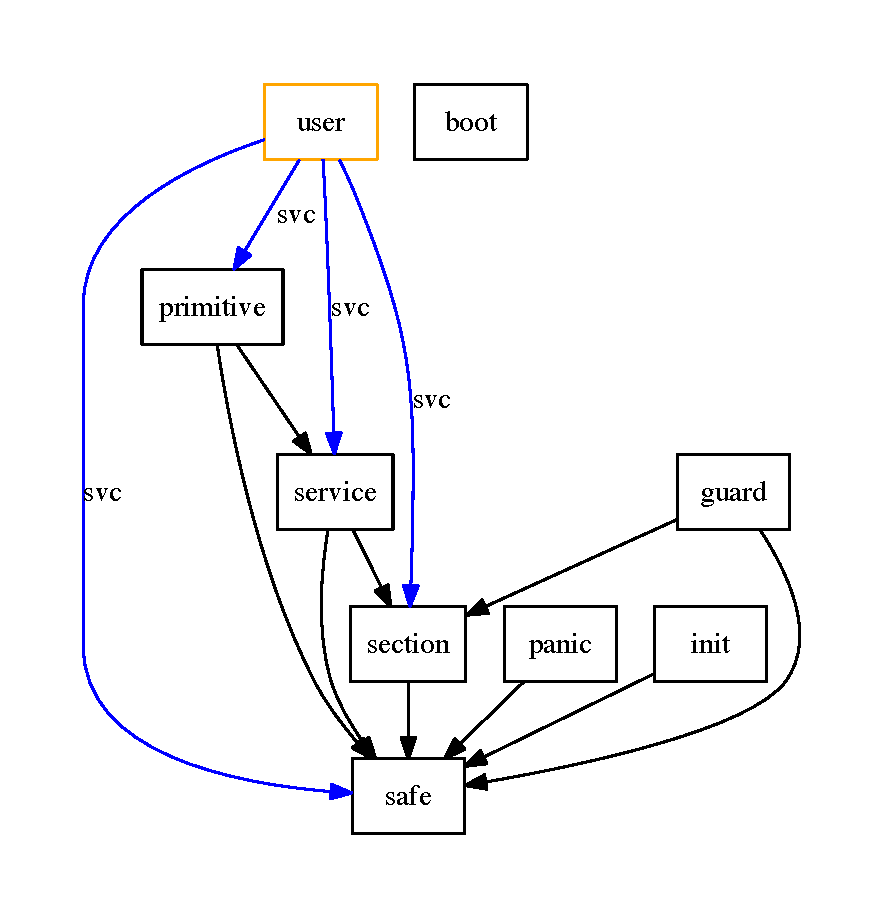
\includegraphics[width=10cm]{chapitres/changement-modes.pdf}
%  \small
%  \begin{tikzpicture}[
%      user/.style ={rectangle, draw=blue, thick, align=center},
%      system/.style ={rectangle, draw=black, thick, align=center},
%      node distance=5mm
%    ]
%    \node [system] (primitive) {\texttt{primitive}};
%    \node [system] (service) [right=of primitive] {\texttt{service}};
%    \node [system] (section) [right=of service] {\texttt{section}};
%    \node [system] (panic) [right=of section] {\texttt{panic}};
%    \node [system] (init) [right=of panic] {\texttt{init}};
%    \node [user] (user) [above=of primitive] {\texttt{user}};
%    \node [system] (boot) [right=of user] {\texttt{boot}};
%    \node [system] (safe) [below=of primitive] {\texttt{safe}};
%    \node [system] (guard) [above=of panic] {\texttt{guard}};
%
%    \draw [->] (primitive) -- (service);
%    \draw [->] (service) -- (section);
%    \draw [->] (service) -- (safe);
%    \draw [->] (section) -- (safe);
%    \draw [->] (primitive) -- (safe);
%    \draw [->] (init) -- (safe);
%    \draw [->] (guard) -- (safe);
%  \end{tikzpicture}
  \caption{Graphe des changements de mode}
  \labelFigure{changementMode}
  \ligne
\end{figure}

Les possibilités de changements de mode sont illustrés par la \refFigure{}{changementMode}.

En mode \plm=user=, on peut appeler une routine \plm=system= déclarée avec le mode \plm=primitive=, \plm=service=, \plm=section= ou \plm=safe=. Appeler une routine \plm=system= est la seule façon de changer de mode d'exécution. L'implémentation de l'appel est réalisé par une instruction de type \emph{Supervisor Call}.

Tous les changements de modes décrits ci-après sont implémentés au moyen d'une instruction classique d'appel de sous-programme.

Les modes \plm=primitive=, \plm=service=, \plm=section= et \plm=safe= sont des modes avec des privilèges décroissants. Aussi, les appels \plm=primitive= -> \plm=service= -> \plm=section= -> \plm=safe= sont valides.

Le mode \plm=boot= est le mode des routines exécutés au démarrage du processeur~; ce mode est isolé.

Le mode \plm=init= est le mode des routines d'initialisation~; le seul changement de mode autorisé est vers le mode \plm=safe=. 

Le mode \plm=panic= est le mode des routines exécutées suite à une panique~; le seul changement de mode autorisé est vers le mode \plm=safe=, car les instructions pouvant engendrer la panique n'y sont pas autorisées. 

Enfin, le mode \plm=guard= est le mode d'évaluation des commandes gardées. On peut y appeler les routines \plm=section= et \plm=safe=.











\sectionLabel{Paramètres formels, arguments effectifs, sélecteurs}{argumentFormel}
\index{Parametre formel@Paramètre formel}
\index{Argument effectif}
\index{Selecteur@Sélecteur}

\subsection{Paramètres formels}

Il existe trois natures de paramètres formels~: \emph{entrée}, \emph{sortie} et \emph{entrée / sortie}, décrits dans le \refTableau{argumentsFormels}. Un sélecteur peut être \emph{anonyme} (par exemple \plm+?+ pour un paramètre formel en entrée), ou comporter un nom (le nom « \texttt{nom} » pour \plm+?nom:+).

Une procédure déclare zéro, un ou plusieurs paramètres formels qui peuvent être en \emph{entrée}, en \emph{sortie} ou en \emph{entrée/sortie}. Une fonction déclare zéro, un ou plusieurs paramètres formels en \emph{entrée}.


\begin{table}[t]
  \centering
  \begin{tabular}{lp{6.5cm}l}
    \textbf{Paramètre formel} & \textbf{Transfert d'information} & \textbf{Sélecteur} \\
    Entrée & Lors de l'appel, de l'appelant vers l'appelé & \plm+?+ ou \plm+?selecteur:+\\
    Sortie & Lors du retour, de l'appelé vers l'appelant & \plm+!+ ou \plm+!selecteur:+\\
    Entrée / sortie & Lors de l'appel, de l'appelant vers l'appelé, et lors du retour, de l'appelé vers l'appelant & \plm+?!+ ou \plm+?!selecteur:+\\
  \end{tabular}
  \caption{Paramètres formels}
  \labelTableau{argumentsFormels}
  \ligne
\end{table}




\subsection{Arguments effectifs}

La syntaxe des différents paramètres formels et de leur argument effectif est résumée dans le \refTableau{argumentsFormelsParametresEffectifs}. 

\begin{table}[t]
  \centering
  \begin{tabular}{llll}
    \textbf{Paramètre formel} & \textbf{Sélecteur} & \textbf{Argument effectif} & \textbf{Sélecteur} \\
    Entrée & \plm+?+         & Sortie & \plm+!expression+ \\
           & \plm+?selecteur:+ & & \plm+!selecteur:expression+ \\
    Sortie & \plm+!+         & Entrée & \plm+?variable+ \\
           & \plm+!selecteur:+ & & \plm+?selecteur:variable+ \\
    Entrée/sortie & \plm+?!+         & Sortie/entrée & \plm+!?variable+ \\
           & \plm+?!selecteur:+ & & \plm+!?selecteur:variable+ \\
  \end{tabular}
  \caption{Paramètre formel et argument effectif}
  \labelTableau{argumentsFormelsParametresEffectifs}
  \ligne
\end{table}









\subsection{Signature d'une routine}

En PLM, une routine est identifiée par son nom et la liste de ses sélecteurs. Il est donc possible de déclarer des routine de mêmes noms, du moment qu'elles se distinguent par le nombre, la nature et le nom des sélecteurs.

[DES EXEMPLES POUR COMPLÉTER] 














 


















\sectionLabel{Fonctions}{defFonction}

Sous le terme \emph{fonction} sont en fait définies les \emph{procédures} et les « vraies » \emph{fonctions}.

Une procédure est appelable dans une instruction et ne peut renvoyer des valeurs que par ses paramètres formels de sortie et d'entrée/sortie.

Une fonction est appelable dans une expression et renvoie une valeur.





\subsectionLabel{Déclaration d'une « vraie » fonction}{declarationFonction}\index{Fonction}

La déclaration d'une fonction est la suivante~:
\begin{PLM}
func mode nom @attribut (arguments_formels) -> $type {
  liste_instructions
}
\end{PLM}
Où~:
\begin{itemize}
  \item \plm=nom= est le nom de la fonction~;
  \item \plm=mode= est le mode associé à la fonction, c'est l'un des mots réservés \plm=primitive=, \plm=service=, \plm=section= ou \plm=safe=~;
  \item \plm=@attribut= est une liste éventuellement vide d'attributs associés à la fonction~;
  \item \plm=arguments_formels= est la liste (éventuellement vide) des paramètres formels~;
  \item \plm=$type= est le type de la valeur renvoyée.
\end{itemize}

Contrairement à beaucoup de langages, PLM n'a pas d'instruction \texttt{return}, qui permettrait de nommer la valeur de retour. En PLM, une variable nommée \plm=result= est implicitement déclarée du type \plm=$type=, et est non valuée initialement. La liste d'instructions de la fonction {\bf doit} valuer cette variable. Sa valeur à l'issue de l'exécution de la liste d'instructions est la valeur renvoyée par la fonction. 
Par exemple~:

\begin{PLM}
func user maFonction @noUnusedWarning () -> $uint32 {
  result = 6
}
\end{PLM}

Ceci définit la fonction \plm=maFonction=, sans argument, appelable uniquement en mode \plm=user=~; l'attribut \plm=@noUnusedWarning= signifie qu'aucune alerte n'est émise si la fonction n'est pas utilisée.

\begin{PLM}
func user autreFonction (?arg:a $uint27 ?b $uint27) -> $uint27 {
  result = a +% b
}
\end{PLM}

Ceci définit la fonction \plm=autreFonction=, avec deux arguments, sans attribut, appelable uniquement en mode \plm=user=.




\subsectionLabel{Déclaration d'une « procédure »}{declarationProcedure}\index{Procédure}

La déclaration d'une « procédure » est la suivante~:
\begin{PLM}
func mode nom @attribut (arguments_formels) {
  liste_instructions
}
\end{PLM}
Où~:
\begin{itemize}
  \item \plm=nom= est le nom de la fonction~;
  \item \plm=mode= est le mode associé à la fonction, c'est l'un des mots réservés \plm=primitive=, \plm=service=, \plm=section= ou \plm=safe=~;
  \item \plm=@attribut= est une liste éventuellement vide d'attributs associés à la fonction~;
  \item \plm=arguments_formels= est la liste (éventuellement vide) des paramètres formels.
\end{itemize}

Aucun type de retour n'est mentionné, aussi aucune variable nommée \plm=result= n'est pré-définie. Une procédure est appelable dans une instruction.










\subsectionLabel{Fonctions requises}{procedureRequise}

La déclaration \plm+required func+ permet de signifier au compilateur qu'une procédure doit être définie, soit par la cible, soit par le programme utilisateur.

Cette déclaration est la suivante~:
\begin{PLM}
required func mode nom @attribut (arguments_formels) -> $type
\end{PLM}

ou~:

\begin{PLM}
required func mode nom @attribut (arguments_formels)
\end{PLM}

Elle consiste en la déclaration de l'en-tête d'une fonction, précédée par le mot réservé \plm+required+.







\subsectionLabel{Fonctions externes}{defProcedureExterne}

Une fonction externe est une procédure définie en C ou en assembleur et appelable en PLM.

La déclaration d'une fonction externe est la suivante~:

\begin{PLM}
extern func mode nom (arguments_formels) -> $type : "nom-assembleur"
\end{PLM}
Où~:
\begin{itemize}
  \item \plm=nom= est le nom de la fonction externe~;
  \item \plm=mode= est la liste non vide de l'ensemble des modes associés à la fonction~;
  \item \plm=@type= est le type de la valeur renvoyée~;
  \item \plm="nom-assembleur"= est le nom qui sera engendré en assembleur, elle correspond à la directive \texttt{asm} de CLANG (et de GCC).
\end{itemize}

Si la fonction externe est en fait une \emph{procédure}, sa déclaration est la suivante~:

\begin{PLM}
extern func mode nom (arguments_formels) : "nom-assembleur"
\end{PLM}

\subsubsection{Exemple de fonction externe}

Prenons l'exemple de cette fonction, qui implémente le blocage de la tâche appelante dans une primitive~:

\begin{PLM}
extern func
primitive block (?!inList:ioWaitingList $taskList) : "blockInList"
\end{PLM}

La signature PLM de cette fonction est \plm=block(?!inList:)=.

Elle est appelable en mode \plm=primitive=, c'est-à-dire dans une primitive. Dans l'instruction d'appel engendré en assembleur, le nom utilisé sera \texttt{func.blockInList}. Le préfixe \texttt{func.} est automatiquement ajouté par le compilateur.

Dans le code C qui implémente cette fonction, la déclaration du prototype est~:

\begin{SHELL}
void block\_in\_list (TaskList * ioWaitingList) \\
asm ("!FUNC!blockInList") ;
\end{SHELL}

Le nom \texttt{block\_in\_list} est interne au code C.

Le type C \texttt{TaskList} correspond au type PLM \plm=$taskList=~; ces deux types sont définis indépendemment, c'est au programmeur de s'assurer qu'ils ont des tailles identiques (ici, 32 bits).

Le mode de passage de l'argument est spécifié par le sélecteur \plm=?!inList:=, c'est le mode \emph{entrée/sortie}, qui correspond au passage d'un pointeur en C. C'est au programmeur de s'assurer que les mode de passage spécifiés en PLM et C correspondent.

Enfin, le nom assembleur de la routine engendrée par le compilateur CLANG est spécifié par la deuxième ligne «~\texttt{asm("!FUNC!blockInList")}~». Le nom « \texttt{blockInList} » doit être celui déclaré comme «~\emph{nom-assembleur}~» dans la déclaration PLM, et « \texttt{!FUNC!} » est remplacé par «~\texttt{func.}~» par le compilateur PLM.





\subsectionLabel{Attribut \texttt{@noUnusedWarning}}{attributFonctionNoWarningIfUnused}\index{"@noUnusedWarning}

L'attribut \plm+@noUnusedWarning+ signifie qu'aucune alerte n'est émise si la fonction n'est pas utilisée.



\subsectionLabel{Attribut \texttt{@exported}}{attributProcGlobale}\index{"@global}

L'attribut \plm+@exported+ signifie que la procédure sera visible par le code C et assembleur du projet. Ainsi une procédure écrite en PLM pourra être appelée à partir du code C et du code assembleur.






\subsectionLabel{Fonctions « universelles »}{fonctionUniverselle}

Les fonctions universelles peuvent être appelées à partir de n'importe quel mode. Leur déclaration est la suivante, la notation de mode est simplement absente~:

\begin{PLM}
// Fonction universelle renvoyant un résultat
func nom @attribut (arguments_formels) -> $type {
  liste_instructions
}
// Procédure universelle
func nom @attribut (arguments_formels) {
  liste_instructions
}
\end{PLM}
Où~:
\begin{itemize}
  \item \plm=nom= est le nom de la fonction~;
  \item \plm=@attribut= est une liste éventuellement vide d'attributs associés à la fonction~;
  \item \plm=arguments_formels= est la liste (éventuellement vide) des paramètres formels~;
  \item \plm=@type= est le type de la valeur renvoyée.
\end{itemize}

En conséquence, les contraintes sur l'écriture de leurs instructions sont importantes~:
\begin{itemize}
  \item comme elles peuvent s'exécuter en mode \plm=user=, seuls les registres de contrôles accessibles dans ce mode sont autorisés~;
  \item comme elles peuvent s'exécuter en mode \plm=safe=, les instructions pouvant engendrer la panique ne sont pas autorisées.
\end{itemize}













\subsectionLabel{Fonctions et registres de contrôle}{fonctionEtRegistresContrôles}

[À REVOIR]

Si la fonction est déclarée avec le mode \plm!user!, seuls les registres de contrôle déclarés \plm!@user! sont accessibles. Dans les autres modes, tous les registres de contrôle sont accessibles.


\subsectionLabel{Fonctions et variables globales}{fonctionEtVariableGlobale}

Voir \refSectionPage{restrictionUsageVariableGlobale}.

%Les fonctions peuvent accéder aux variables globales en lecture, mais ne peuvent pas les modifier.
%
%L'accès en lecture à une variable globale est autorisé par la variable qui nomme la fonction parmi les routines autorisées~:
%
%\begin{PLM}
%var gGlobalVar $uint56 {
%  ...
%  func getGlobalVar
%}
%
%func getGlobalVar user () -> $uint56 {
%  result = getGlobalVar
%}
%\end{PLM}
%



















\sectionLabel{Routines système}{declarationSystem}\index{system}

Une \emph{routine système} est une routine qui s'exécute dans un des modes \plm=primitive=, \plm=service=, \plm=section= ou \plm=safe=. Elle est appelable à partir des modes~:
\begin{itemize}
 \item \plm=user=, l'appel s'effectue alors à travers une instruction \emph{Supervisor Call}~;
  \item d'un autre mode privilégié, en respectant le graphe de la \refFigurePage{}{changementMode} (l'appel est alors une instruction d'appel de sous-programme).
\end{itemize}

Comme une \emph{routine système} est exécutée par le processeur en mode privilégié, les registres de contrôles accessibles.




\subsection{Déclaration d'une routine système}


La déclaration d'une routine système est la suivante~:
\begin{PLM}
system mode nom @attribut1 @attribut2 (arguments_formels) {
  liste_instructions
}
\end{PLM}
Où~:
\begin{itemize}
  \item \plm=nom= est le nom de la routine système~;
  \item \plm=mode= est le mode associé à la routine, c'est l'un des mots réservés \plm=primitive=, \plm=service=, \plm=section= ou \plm=safe=~;
  \item \plm=@attribut1= \plm=@attribut2= est une liste éventuellement vide d'attributs associés à la routine système~; actuellement, seul l'attribut \plm!@noUnusedWarning! est défini (\refSubsectionPage{attributNoWarningIfUnusedSection}).
\end{itemize}










\subsectionLabel{Attribut \texttt{@noUnusedWarning}}{attributNoWarningIfUnusedSection}\index{"@noUnusedWarning}

L'attribut \plm+@noUnusedWarning+ signifie qu'aucune alerte n'est émise si la section n'est pas utilisée.




















\sectionLabel{Routines d'interruption}{declarationRoutineInterruption}\index{Routine!Interruption}\index{Interruption!Routine}

La déclaration d'une routine d'interruption est la suivante~:
\begin{PLM}
system mode nom {
  liste_instructions
}
\end{PLM}
Où~:
\begin{itemize}
  \item \plm=nom= est le nom de la routine~;
  \item \plm=mode= est le mode associé à la routine, c'est l'un des mots réservés \plm=service=, \plm=section= ou \plm=safe=.
\end{itemize}

Le nom de la routine doit être un des noms de routines d'interruption déclarés par la déclaration \plm=target= (voir §§).

Le mode d'exécution associé est l'un des trois modes suivants~:
\begin{itemize}
  \item \plm=service=, les routines de l'exécutif rendant des tâches prêtes peuvent être appelées~;
  \item \plm=section=, la routine d'interruption n'interfère pas avec l'exécutif~;
  \item \plm=safe=, comme pour \plm=section=, et de plus les instructions pouvant engendrer la panique y sont interdites.
\end{itemize}









\section{Routines utiles}

Le compilateur élimine les routines qui ne sont jamais appelées, en calculant le graphe des appels. Les racines de ce graphe sont les procédures requises (\refSubsectionPage{procedureRequise}), les routines \plm=boot=, \plm=init= et \plm=panic=. Les routines inatteignables sont éliminées, sans message d'alerte pour les routines déclarées avec l'attribut \plm!@noUnusedWarning!.











\sectionLabel{Récursivité}{routinesRecursives}\index{Routines!recursives@récursives}

Par défaut, le compilateur émet un message d'erreur si une ou plusieurs routines récursives sont détectées. L'option \OPTION{-{}-do-not-detect-recursive-calls} (\refSectionPage{optionCodeEngendre}) permet d'inhiber cette recherche.

L'option \OPTION{-{}-routine-invocation-graph} permet d'obtenir un fichier contenant le graphe d'invocation, qui peut être affiché par le logiciel \texttt{graphviz}\index{graphviz}. Si le fichier source est \texttt{source.plm}, le fichier engendré s'appelle \texttt{source.subprogramInvocation.dot}.

